\documentclass[12pt]{article}
 \usepackage{fontspec}
 \usepackage[english]{babel} 
 \newfontfamily\skt[Script=Devanagari]{Siddhanta}
 \usepackage{parskip}
 \usepackage[dvipsnames]{xcolor}
 \usepackage{graphicx}
\graphicspath{ {images/} }
\usepackage{float}
\usepackage{wrapfig}
\usepackage{array}
\title{\textbf{The Sāvitrī and the upāsanā of the Deva Savitṛ}}
\author{Bhārgavaḥ }
\date{}

\begin{document}
\maketitle

\begin{center}
{\skt
॥ भ॒द्रं नो॒ अपि॑ वातय॒ मनः॑ ॥\\
॥ देव॑ सवितः॒ प्रसु॑व ॥\\
॥ वि॒दा मघ॑वन् विदो३म् ॥
}\\
 \end{center}

\section{The mantra-s} 
The Sāvitrī is the core mantra used in Savitrupāsanā. It also has other notable deployments, which will be described later. Its ṛṣi is Viśvāmitra of the clan of Gāthin, the chandas is nicṛd gāyatrī and the devatā is Savitṛ. It is from the $3^{rd}$ maṇḍala of the Ṛgveda (RV 3.62.10). The meter is termed  nicṛd gāyatrī because the syllable count is 23, one short of the usual 24 for a gāyatrī. This arises due to the intrinsic saṃdhi, which creates {\skt वरेण्यम्} from {\skt वरेणियम् }. The Sāvitrī goes thus:\\
{\skt
तत् स॑वि॒तुर् वरे॑ण्य॒म् भर्गो॑ दे॒वस्य॑ धीमहि । धियो॒ यो नः॑ प्रचो॒दया॑त् ॥
}\\[10pt]
Given the popularity of the Sāvitrī it is common to see numerous translations of the same; however, these often do not get certain aspects of the Old Vedic register of Sanskrit. It is important that one does the japa of this mantra with a proper grasp of its sense in the original language. Hence, we provide a translation of the mantra in full here.\\[8pt]
tat= that; Savituḥ= of Savitā; vareṇyam= excellent or desirable; bhargaḥ= radiance (neuter accusative); devasya= of the god; dhīmahi= may we fix [our mind]/ may we focus on; dhiyaḥ= insights (plural of dhī); yaḥ= who; nas= our; pracodayāt= may he inspire.\\
There are a few key points to make note of: first, the verb form dhīmahi; this is the āśīr-liṅ (benedictive) 1st person plural form of the root dhā, which belongs to class 3 (juhotyādi gaṇa). We are unaware of the occurrence of other āśīr-liṅ forms of the verb dhā in the RV. It is used symmetrically with the 3rd person singular āśīr-liṅ form of the verb pra-cud i.e. pracodayāt. These forms are not commonly used outside of such mantra-s suggesting that it was an ancient usage of a verb-pair presenting a relationship between the worshipers (dhīmahi) and the god (pracodayāt). Second, the name of the god Savitṛ is commonly combined with the word deva (god). This combination probably again has an ancient connotation, which is reflected in theonyms of other Indo-European branches like proto-Germanic *Tiwaz>Tyr. It (theos) was probably also used in this sense for the Greek Hyperion\footnote{A Titan, even as Savitṛ is also called Asura in the RV}, the likely cognate of Savitṛ, in the Homeric language. Third, the word dhiyaḥ, has been specifically chosen for alliteration with dhīmahi\footnote{Word analysis suggests that Viśvāmitra had a particular propensity for alliterative or polyptotonic usages such as the āmreḍita. See: A note on āmreḍita-s in the Ṛgveda and issues of word distribution https://manasataramgini.wordpress.com/2018/05/14/a-note-on-aṃreḍita-s-in-the-ṛgveda-and-issues-of-word-distribution/}. It means not just any thought but specifically inspired thought or insight that leads to the ``seeing'' of special knowledge, such as that embodied in a Vedic mantra. Thus, we get,\\[8pt]
May we focus on the excellent radiance of the deva Savitṛ who will inspire our insights.\\[10pt]
The Sāvitrī is prefixed with the three vyāhṛti-s for the actual japa. \\
{\skt भूर् भुवः सुवः ।
}\\
The three basic vyāhṛti-s are to understood as the three realms, the earth, the atmosphere and the heavens, which are pervaded by the light of the god Savitṛ. These are given above in the Yajurvedic form, which may also be followed in Atharvavedic tradition. In the Ṛgvedic tradition the internal saṃdhi is enacted and we have {\skt स्वः } for {\skt सुवः}. The mysteries of these vyāhṛti-s are explained, among other places, in the Taittirīya-śruti. \\[10pt]
 For the practice of prāṇāyāma, it is prefixed with the 7 vyāhṛti-s.\\
{\skt ॐ भूः । ॐ भुवः । ओग्ँ सुवः । ॐ महः । ॐ जनः । ॐ तपः । ओग्ँ सत्यम् ।
}\\
These may be understood as a larger set of 7 regions of space, which are pervaded by the light of Savitṛ. The nasals preceding sa are given as per the Yajurvedic tradition. They are rendered as the usual nasals in the RV and AV traditions.\\[10pt]
It suffixed by the incantation known as the brahmaśiras.\\
{\skt ॐ आपो॒ ज्योती॒ रसो॒ ऽमृतं॒ ब्रह्म॒ भूर्-भुव॒-सुव॒रो३म् ॥
}\\
Here, āpaḥ= waters; jyotiḥ= light; rasaḥ= life fluids; amṛtaṃ= immortality; brahma= mantra-power. bhūḥ, bhuvaḥ and suvaḥ and the three main vyāhṛti-s \\[10pt]
Then there is the four-footed form which is a mystery teaching in the śruti of the Śukla-yajurvedin-s. This is obtained by adding the below.\\
{\skt प॒रो-र॑जसे॒ ऽसाव॒दो३म् ॥
}\\
This technically converts it into an anuṣṭubh due the addition of 8 additional syllables. In the mystery teaching it is termed the beautiful or the vivid foot that is beyond the immediate space (rajas: see section below for details). In the same teaching it is revealed that the $4^{th}$ foot is a critical aspect of both abhicārika and vṛddhi deployments of the Sāvitrī. Indeed, combined with the teaching of Śaunaka it might be deployed along with the Sāvitrī with syllables inverted (viparīta-prayoga) for abhicārika purposes.\\[10pt]
The Atharvan tradition gives a saṃpuṭikaraṇa of the Sāvitrī known as the Mahāsāvitrī. It goes thus:\\[8pt]
{\skt 
ॐ भूः । ॐ भुवः । ॐ स्वः । ॐ महः । ॐ जनः । ॐ तपः । ॐ स॒त्यं । ॐ तत् स॑वि॒तुर् वरे॑ण्य॒म् भर्गो॑ दे॒वस्य॑ धीमहि । धियो॒ यो नः॑ प्रचो॒दया॑त् ॥ ॐ आपो॒ ज्योती॒ रसो॒ ऽमृतं॒ ब्रह्म॒ भूर्-भुव॒-सुव॒रो३म् ॥ ॐ भूर्-भुवः-सुवर्-महर्-जनस्-तपः सत्यं मधु॑ क्षरन्ति । ॐ आपो॒ ज्योती॒ रसो॒ ऽमृतं॒ ब्रह्म॒ भूर्-भुव॒-स्वरो३म् । ओम्॑ तद्-ब्र॒ह्म । ओम्॑ तद्-वा॒युः । ओम्॑ तद्-आ॒त्मा । ओम्॑ तत्-स॒त्यम् । ओम्॑ तत्-सर्वम्॑ । ओम्॑ तत्-पुरों॒ नमः ॥
}\\[8pt]
Some hold that deploying this form of the mantra $10 \times$ can be considered an equivalent of deploying the regular version $108 \times$. This mantra is also seen as a combination of that of the gods Savitṛ and Vayu. These two are an ancient pair as indicated by the Mṛgāra mantra-s. Savitṛ pervades space with light, while the Vayu pervades it as the rarefied substance and the force which holds the celestial bodies together. These two thus form the foundation of existence.\\[10pt]
The Atharvan tradition also teaches the mystery deployment, which adds the Atharvaśiras comprised of the Atharvanic high vyāhṛti-s.\\[8pt]
{\skt 
ॐ भुर्-भुवः-स्वः । ॐ तत् स॑वि॒तुर् वरे॑ण्य॒म् भर्गो॑ दे॒वस्य॑ धीमहि । धियो॒ यो नः॑ प्रचो॒दया॑त् ॥ ॐ भूर् भुवः स्वर् जनद् वृधत् करद् रुहन् महत् तच् छम् ओम् ॥
}\\[8pt]
Here, the vyāhṛti-s janad, vṛdhat, karat, ruhat, mahat, tat, śam and oṃ are the special vyāhṛti-s of the Bhṛgvāṅgiras. These are part of the secret teaching of the Atharvan. The knower of the Bhṛgvāṅgirasa-śruti may use this deployment to protecting himself while attacking his enemies with the stoma-bhāga-prayoga.\\[10pt]
The viparīta-prayoga (inverse deployment) is specified for abhicārika purposes.\\
{\skt
त्यादचोप्र नो यो योधि । हिमधी यस् व दे गोर्भ । म्यणिरेव तुर्विस त्त ॥
}\\
A variant inverse deployment involves merely inverting the three feet.\\
{\skt
धियो॒ यो नः॑ प्रचो॒दया॑त् । भर्गो॑ दे॒वस्य॑ धीमहि । तत् स॑वि॒तुर् वरे॑णि॒यों ॥
}

\section{The mysteries}
The śruti of the the Vājasaneyin-s provides a mystery teaching regarding the Sāvitrī, which associates the 3 feet of the core mantra with a triad of triads, which is summarized below.
 \begin{center}
 \begin{tabular}{|| c | c  | c ||} 

{\skt भूमिः} & {\skt अन्तरिक्षम्} & {\skt द्यौस्}\\
{\skt ऋचः}  & {\skt यजूंषि}  & {\skt सामानि}  \\
{\skt प्राणः}  & {\skt अपानः}   &{\skt व्यानः}  \\
\end{tabular}
\end{center}
The one who meditates on the Sāvitrī with this knowledge is understood as penetrating the realms of the universe with the first triad, the realms of Veda-s with the second triad and realms of life with the the third triad. The fourth foot is said to blaze beyond the expanse of the visible space, the ``rajas'' and its knowledge confers splendor.\\[10pt]
The Atharvan tradition holds (the teaching of Maudgalya to Glāva Maitreya)  that the Sāvitrī is pervaded by the god Deva Savitṛ and his consort Sāvitrī in the form of 12 pairs of forms corresponding to each syllable  (Figure \ref{fig:fig1}). In these forms the two deities pervade the universe and the ritual. This presentation in the Atharvan tradition is consistent with the statement of Vāmadeva Gautama in the RV: {\skt आप्रा॒ रजां॑सि दि॒व्यानि॒ पार्थि॑वा॒} in RV 4.53.3, i.e. celestial and the earthly realms. The three feet of the Sāvitrī are described giving rise to three sequences of emanations that culminate in the ritual observance of the brāhmaṇa (Figure \ref{fig:fig1}; lower panel). The ritualist who performs the deployment of the Sāvitrī with the appropriate knowledge of the omniform manifestation of Savitṛ and his consort and the emanations of the three feet meets with success.\\
 % Figure 1
 \begin{figure}[h]
  \centering
    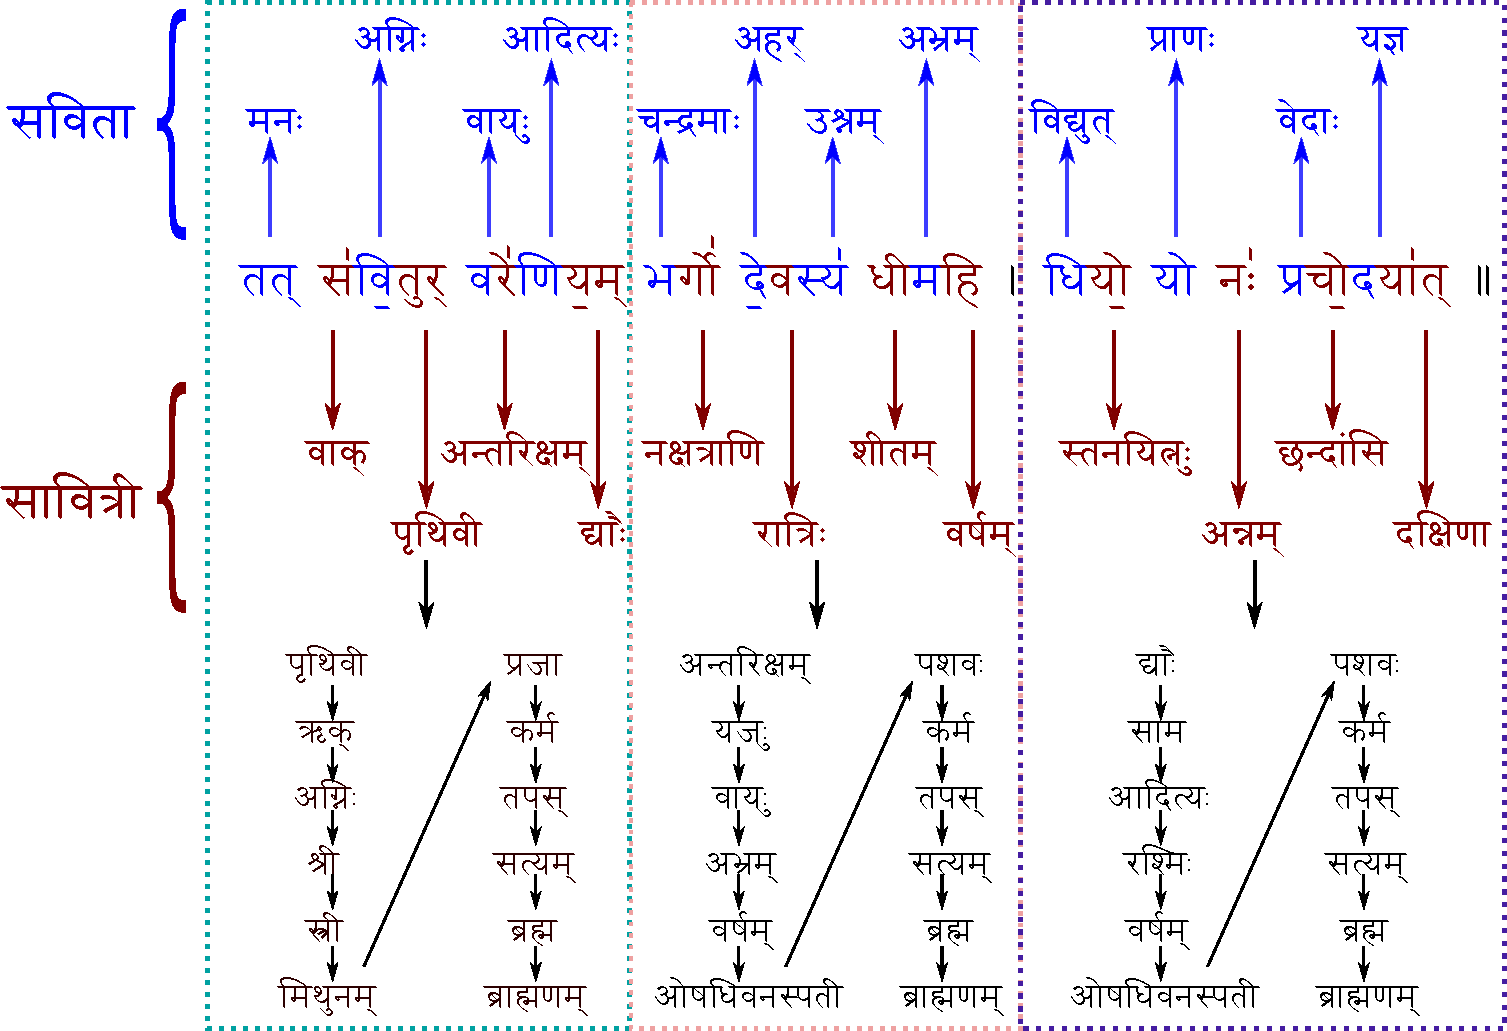
\includegraphics[width=\textwidth]{savitri_fig1}
    \caption{The structure and the emanations of the Sāvitrī as per the Atharvan tradition}
    \label{fig:fig1}
    \end{figure}

\section{The prayoga-s}
 \begin{enumerate}
\item The ritual of ācamana. He sips water $3\times$ with the 3 feet of the Sāvitrī. Thereafter, he performs mārjanam at the appropriate spots on the face and one shoulder with the feet of the āpohiṣṭhiya mantra-s, at other shoulder with the 7 vyāhṛtis, at the chest with the whole sāvitrī and on the head with the brahmaśiras. He may use this ācamana for routine smārta and ekāgni purposes. The only exceptions are Atharvan rituals (where he should use the Atharvavedīya ācamana-vidhi) and the three-fire śrauta rituals.
\item The Sāvitrī is the essential mantra for the twilight saṃdhyopāsanā or the worship of the god Savitṛ during the day. Every dvija has to receive this mantra from his father or male guardian during his upanayana. If a brāhmaṇa male does not perform this rite at all then the king who observes dharma may employ him a śūdra. He should first take a bath if he is an state of impurity before performing the Savitropāsanā. Beyond a bath with water, a dvija should also perform prokṣaṇa. Having deployed the saṃdhyā preliminaries as ordained in his śruti or that ordained by in the Baudhāyana tradition, he can perform the mantra-practice. He does japa (inaudibly) of the Sāvitrī $1008 \times$ or $108 \times$. If he does not have the time he may perform prāṇāyama with the 7 vyāhṛti-s and the brahmaśiras $10 \times$. The most simple form of prāṇāyāma involves inhaling with oṃ bhūḥ. Retaining the breath with the rest of the mantra and exhaling with the brahmaśiras. After concluding the japa or prāṇāyāma he offers arghya $3\times +1$ for expiation with his cupped palms or a shell. He then invokes Mitra (morning) and Varuṇa (evening) or both if he has missed one. Then he utters the purificatory incantation of Agni, Sūrya or the waters.
\item If a dvija has committed a ghora-pāpa, e.g. abortion, brāhmaṇī-gamanam, puṃścalī-gamanam etc, or has killed a dog, a beaver, a mongoose, a goose or a garden lizard, then he may purify himself after reciting the Sāvitrī $8000\times$ continuously starting before the sun rises. If a dvija has had his bath but is uncertain of his ritual purity due to activities he has performed since his bath, he may wear new clothes and perform a japa of the Sāvitrī for a fixed number of times or do prāṇāyāma as described above. Then he recites the following incantation of Vasiṣṭha:\\[8pt]
{\skt 
शुची॑ वो ह॒व्या म॑रुतः॒ शुची॑नां॒ \\
शुचिं॑ हिनोम्य् अध्व॒रं शुचि॑भ्यः ।\\
ऋ॒तेन॑ स॒त्यम् ऋ॑त॒साप॑ आय॒ञ् \\
 छुचि॑जन्मानः॒ शुच॑यः पाव॒काः ॥
}\\[8pt]
Pure oblations to you O Marut-s, the pure ones;\\
A pure ritual I offer to the pure ones;\\
By the ṛta the ṛta-knowers have attained truth,\\
of pure birth, they who are pure, the purifiers.\\
\item After the conclusion of upāsanā the ritualist must invoke Savitṛ for protection. He sprinkles water on the place where he did is upāsanā and having touched the ground with his ring finger, he touches the spot between his eyebrows with the same finger. While doing this action he recites the following Sāvitra incantations of Śyāvāśva Ātreya:\\[8pt]
{\skt
अ॒द्या नो॑ देव सवितः प्र॒जाव॑त् सावीः॒ सौभ॑गम् । परा॑ दु॒ष्ष्वप्न्यं॑ सुव ॥\\
विश्वा॑नि देव सवितर् दुरि॒तानि॒ परा॑ सुव । यद् भ॒द्रं तन् न॒ आ सु॑व ॥
}\\[8pt]
Today, god Savitṛ, you have impelled to us a good share consisting of offspring. Impel away the bad dream.\\
O god Savitṛ  impel away all difficulties; what is auspicious,  impel that here to us\footnote {These are also the mantra-s with which the Vaiśvadeva-śastra is initiated in the śrauta ritual. The Hindu freedom fighter of Rām Prasād Bismil when being executed by the English was asked for his last wish. To which he replied: ``The downfall of the British Empire.'' Then he invoked Savitṛ reciting these mantra-s as he was taken to the noose. They supposed to be for him to be reborn to fight the English again and the reborn Indian nation}.
\item The rite of the herb-mixture taught by the sage Uddālaka Āruṇi to his student Yājñavalkya Vājasaneya. 
\begin{itemize}
\item He performs the preparatory vrata of 12 days during which he controls his diet and observes celibacy.
\item The rite is done during uttarāyaṇa on an auspicious day of the waxing phase of the moon when it is in a male constellation after his regular evening rituals and before sleeping. 
\item He takes all kinds of plants and fruits and grinds them into a mixture with a little bit off butter in a bowl made of fig-wood or metal
\item He then prepares the fire altar by cleaning and wiping. Then he makes the initial ghee offering using a darvi at the svāhā with the mantra:\\[8pt]
{\skt याव॑न्तो देवास्॒ त्वयि॑ जातवेदस् ति॒र्यञ्चो॒ घ्नन्ति॒ पुरु॑षस्य॒ कामा॑न् । तेभ्यो॒ ऽहं भ॑ग॒धेयं॑ जुहोमि॒ ते मा॒ तृप्ताः॒ सर्वैः॒ कामै॑स् तर्पयन्तु॒ स्वाहा॑ । या ति॑रश्ची नि॒पद्य॑ते॒ ऽहं वि॑धर॒णी इ॑ति । तां त्वा॑ घृ॒तस्य॒ धार॑या॒ यजे॒ सग्ँरा॑धनीम् अहग्ँ॒ स्वाहा॑ ॥
}
\item He then makes the long series of ghee offerings  with the yajus mantra-s:\\[8pt]
{\skt ज्ये॒ष्ठाय॒ स्वाहा॒ श्रेष्ठा॑य॒ स्वाहा॑ ॥ प्रा॒णाय॒ स्वाहा॒ वसि॑ष्ठायै॒ स्वाहा॑ ॥ वाचे॒ स्वाहा॑ प्रति॒ष्ठायै॒ स्वाहा॑ ॥ चक्षु॑षे॒ स्वाहा॑ सं॒पदे॒ स्वाहा॑ ॥ श्रोत्रा॑य॒ स्वाहा॒ऽऽयत॑नाय॒ स्वाहा॑ ॥ मन॑से॒ स्वाहा॒ प्रजा॑त्यै॒ स्वाहा॑ ॥ रेत॑से॒ स्वाहा॑ ॥ अ॒ग्नये॒ स्वाहा॑ ॥ सोमा॑य॒ स्वाहा॑॥ भूः॒ स्वाहा॑ ॥ भुवः॒ स्वाहा॑॥ स्वः॒ स्वाहा॑ ॥ भूर् भु॒वः स्वः॒ स्वाहा॑ ॥ ब्र॑ह्मणे॒ स्वाहा॑ ॥ क्ष॒त्राय॒ स्वाहा॑ ॥ भू॑ताय॒ स्वाहा॑ ॥ भवि॒ष्यते॒ स्वाहा॑ ॥ विश्वा॑य॒ स्वाहा॑ ॥ सर्वा॑य॒ स्वाहा॑ ॥ प्र॒जाप॑तये॒ स्वाहा॑ ॥
}\\[8pt]
After each distinct offering (marked by a double daṇḍa), whatever ghee remains behind in the darvi he pours into the herb mixture and stirs it  up. 
\item Touching the bowl with the mixture with his right hand and holding his left hand to his chest he recites the following incantation:\\[8pt]
{\skt भ्रम॑द् असि । ज्वल॑द् असि । पू॒र्णम् अ॑सि । प्र॒स्त॒ब्धम् अ॑सि । ए॒क॒स॒भम् अ॑सि । हि॒ङ्कृ॒तम् अ॑सि । हि॒ङ्क्रि॒य॒मा॒नम् अ॑सि । उ॒द्गी॒थम् अ॑सि । उ॒द्गी॒य॒मा॒नम् अ॑सि । श्रा॒वित॑म् असि । प्र॒त्या॒श्रा॒वि॒तम् अ॑सि । आर्द्रे॑ संदी॒प्तम् अ॑सि । वि॒भूर् अ॑सि । प्र॒भूर् अ॑सि । अन्न॑म् असि । ज्योति॑र् असि । नि॒धन॑म् असि । सं॒वर्गो॑ ऽसि ॥ अथै॑न॒म् उद्य॑च्छ॒त्य् आम॒ग्ँस्य् आम॑ग्ँ हि ते॒ महि॑ । स॒ हि॒ रा॒जेशा॒नो ऽधिपतिः ।स॒ मा॒ग्ँ राजेशा॒नो ऽधि॑पतिं करोतु ॥
}
\item He then consumes the mixture as an offering to Savitṛ within him in three courses each with the following incantation (the feet of the Sāvitrī are silently muttered in each case):\\[8pt]
{\skt ॐ तत् स॑वि॒तुर् वरे॑ण्य॒म् । मधु॒ वाता॑ ऋताय॒ते मधु॑ क्षरन्ति॒ सिन्ध॑वः । माध्वी॑र् नः स॒न्त्व् ओषधीः॑ । भूः॒ स्वाहा॑ ॥
}\\[8pt]
{\skt भर्गो॑ दे॒वस्य॑ धीमहि । मधु॒ नक्त॑म् उ॒तोषसि॒ मधु॑म॒त् पार्थि॑वग्ँ रजः । मधु॒ द्यौर् अ॑स्तु नः पि॒ता । भुवः॒ स्वाहा॑ ॥
}\\
{\skt धियो॒ यो नः॑ प्रचो॒दया॑त् । मधु॑मान् नो॒ वन॒स्पति॒र् मधु॑माग्ँ अस्तु॒ सूर्यः॑ । माध्वी॒र् गवो॑ भवन्तु नः । स्वः॒ स्वाहा॑
}\\[8 pt]
He then recites (Sāvitrī is muttered in silence):\\[8pt]
{\skt ॐ भुर्-भुवः-स्वः । ॐ तत् स॑वि॒तुर् वरे॑ण्य॒म् भर्गो॑ दे॒वस्य॑ धीमहि । धियो॒ यो नः॑ प्रचो॒दया॑त् ॥ मधु॒ वाता॑ ऋताय॒ते मधु॑ क्षरन्ति॒ सिन्ध॑वः । माध्वी॑र् नः स॒न्त्व् ओषधीः॑ ।  मधु॒ नक्त॑म् उ॒तोषसि॒ मधु॑म॒त् पार्थि॑वग्ँ रजः । मधु॒ द्यौर् अ॑स्तु नः पि॒ता । मधु॑मान् नो॒ वन॒स्पति॒र् मधु॑माग्ँ अस्तु॒ सूर्यः॑ । माध्वी॒र् गवो॑ भवन्तु नः । अहम् एवे॑द॒ग्ँ सर्वं॑ भूयासं भूर् भु॒वः स्वः॒ स्वाहा॑ ॥
}\\[8pt]
He then sips some water and washes his hands and sleeps behind the fire altar with his head to the East. 
\item He the wakes up the next day and utters the following incantation looking at the sun.\\[8pt]
{\skt दि॒शाम् ए॒कपु॑ण्डरी॒कम् अ॑सि ।
अ॒हं म॒नुष्या॑णाम् एकपुण्डरी॒कं भू॑यासम् ॥
}
\item He then silently recites the lineage of teachers of this rite:\\[8pt]
{\skt
उद्दालक आरुणिर् याज्ञवल्क्यो वाजसनेयो मधुकः पैङ्ग्यश् चूलो भागवित्तिर् जानकिर् आयस्थूणः सत्यकामो जाबालिः॥
}
\item If he has seen a beautiful woman in his dream that night then his rite is a success.
\end{itemize}
 \end{enumerate}

\section{Appendices}
\subsection{Alternative Sāvitrī-s?}
Today the Sāvitrī is universally used by all dvija-s for their saṃdhyopāsanā/ Savitrupāsanā. However, we know that the saṃdhyā rite goes back to at least the Indo-Iranian period. This raises the question as to whether there was a Savitrupāsanā before the extant Sāvitrī was composed by Viśvāmitra. It is notable that Viśvāmitra himself specifically mentions that the god is worshiped 3 times in a day.\\[8pt]
{\skt हिर॑ण्यपाणिः सवि॒ता सु॑जि॒ह्वस् त्रिर् आ दि॒वो वि॒दथे॒ पत्य॑मानः ।\\
दे॒वेषु॑ च सवितः॒श्लोक॒म् अश्रे॒र् आद् अ॒स्मभ्य॒म् आ सु॑व स॒र्वता॑तिम् ॥
}RV 3.54.11\\[8pt]
Golden-handed Savitṛ with a good  tongue, three times a day in the ordained [ritual] being the lord,\\
among the gods you O Savitaḥ have set your call, now impel to us the totality [of prosperity].\\[8pt]

Then again he states:\\[8pt]
{\skt त्रिर् आ दि॒वः स॑वि॒ता सो॑षवीति॒ राजा॑ना मि॒त्रावरु॑णा सुपा॒णी ।
}RV 3.56.7 \\[8pt]
Thrice a day Savitṛ repeatedly impels [with] the two kings, Mitra and Varuṇa, of good hands.\\[8pt]
We take the above references to the rite ordained thrice a day to be none other than an ancient version of the extant Savitrupāsanā, especially given that he mentions Mitra and Varuṇa, who also receive worship at the twilights along with Savitṛ. Now Viśvāmitra is not the only sage who mentions the rite of Savitṛ performed 3 times a day. Vāmadeva Gautama alludes to it too:\\[8pt]

{\skt ये ते॒ त्रिर् अह॑न् सवितः स॒वासो॑ दि॒वे-दि॑वे॒ सौभ॑गम् आसु॒वन्ति॑ ।
}RV 4.54.6\\[8pt]
O Savitaḥ, thrice a day your impulsions are those which impel good fortune day after day\\[8pt]
Hence, we suspect that the three-fold daily Savitrupāsanā was already a prevalent form of worship even in the days of the RV and not started by Viśvāmitra for the first time. This mantra-practice was also likely associated with the repeated allusion to the śloka or the call of Savitṛ, which marked these transition points of the day. From a study of the RV it appears that several families might have originally had mantra-s comparable to the Vaiśvāmitra Sāvitrī, which later became universal. The mantra-s presented below are examples of themes parallel to the Sāvitrī in the compositions of other clans:\\[8pt]
{\skt  तद् राधो॑ अ॒द्य स॑वि॒तुर् वरे॑ण्यं व॒यं दे॒वस्य॑ प्रस॒वे म॑नामहे ।
}RV 1.159.5\\[8pt]
Today we shall meditate on that excellent favor/power of the Deva Savitṛ at [his] impulse.\\[8pt]
{\skt  तत् स॑वि॒तुर् वृ॑णीमहे व॒यं दे॒वस्य॒ भोज॑नम् ।\\
श्रेष्ठं॑ सर्व॒धात॑मं॑ तुर॒म् भग॑स्य धीमहि ॥
} RV 5.82.1\\[8pt]
We chose that enjoyment of Deva Savitṛ; may we focus on Bhaga's best all-giving power.\\[8pt]
{\skt दे॒वस्य॒ श्लोकं॑ सवि॒तुर् म॑नामहे ॥
} RV 7.82.10\\[8pt]
We meditate upon the call of  deva Savitṛ.\\[8pt]
{\skt श्रेष्ठे॑ स्याम सवि॒तुः सवी॑मनि॒ तद् दे॒वाना॒म् अवो॑ अ॒द्या वृ॑णीमहे ॥
} RV 10.36.12\\[8pt]
May we be in the best impulsion of Savitṛ: that aid of the gods we choose today.\\[8pt]
Some of these mantra-s use the word {\skt अद्य}, i.e. today, perhaps suggesting that the rite was done daily. They are conceptually similar to the Sāvitrī in choosing meditating or focusing on the impulsion or the power of the god.

\subsection{Rajāmsi}
The fourth foot of the Sāvitrī implies that Savitṛ shines from beyond the rajas. What is this rajas, or more precisely the rajāmsi, since the Veda knows of a plurality of them. Vāmadeva Gautama says:\\[8pt]
{\skt त्रिर् अ॒न्तरि॑क्षं सवि॒ता म॑हित्व॒ना त्री रजां॑सि परि॒भुस् त्रीणि॑ रोच॒ना ।\\
ति॒स्रो दिवः॑ पृथि॒वीस् ति॒स्र इ॑न्वति त्रि॒भिर् व्र॒तैर् अ॒भि नो॑ रक्षति॒ त्मना॑ ॥
}\\[8pt]
Savitṛ [encompasses] the atmosphere thrice by his greatness; he encompasses the three rajas realms and the three rocana realms.\\
He drives the three heavenly and the three earthly realms [and] with three-fold laws he protects us by himself.\\[8pt]
While there is a clear emphasis on the tripartation in this mantra, the multiplicity of realms of the old Hindu cosmography is evident here. The rajāmsi are clearly distinct from the atmospheric realm (antarikṣa) and the realms of light (rocana). The rajas realms are also mentioned as being precisely measured out by the strides of Viṣṇu (e.g. RV 6.49.13; 1.154.1) and are again described as being 3 in number in this context (e.g. RV 6.49.13 ). In the sūkta of Śyāvaśva Ātreya (RV 5.81) it becomes clear that Savitṛ performs a similar function of mensuration of these realms. One may say that this function of Viṣṇu goes back to the beginning of cosmic time, while that of Savitṛ apparently happens on a daily basis. Indeed, the two deities are offered combined oblations in the Pratha-Sapratha offerings related to the super-heated gharma pot of the old Pravargya ritual (RV 10.181).  From these references, we can infer that the old ārya-s saw the earthly realm as surrounded by the antarikṣa-s i.e. the atmospheric realms, followed by the  rajāmsi ``near space'', and then the still more distant celestial realms, the rocana-s and div-s. The light of the sun was seen as coming from beyond the rajāmsi and Savitṛ is explicitly associated with this light. Thus, the sun may be seen as marking the beginning of the rocana realms (see also RV 10.189.2) or those of light, which include the realms of the stars. The div-s are seen as three too. Of them two are explicitly described as being under Savitṛ (upastha) while one belongs to the death-dealing Yama (RV 1.35.6). The sun is alluded as being in one of these div-s.  In RV 1.35.9 is stated that the div is reached via the black rajas realms. These allusions suggest that the rocana-s and the div-s are essentially equivalent. In conclusion, it might be mentioned that the Vedic cosmography was rather elaborate and has been poorly understood due to the assumption that it might have been unsophisticated (barring Lokamanya Tilak's musings in this regard).

\subsection{Deva Savitṛ}
While the Sāvitrī remains a popular mantra among modern Hindus, most of them do not know its deity. Even of those who know Savitṛ to be the deity, few have a clear idea of the nature of this god. Most believe that he is none other than the Sun of our solar system. Yet, the RV is quite clear about him not being the same as the sun. The sun is merely one manifestation of his activity. In particular, he is specifically linked to the celestial lights, like the rays of the sun (e.g. RV 1.35.7; 4.14.2; 5.81.4; 10.139.1) \footnote{It is in this context that the famed Vijayanagaran scholiast Sāyaṇa gives a large value that may be interpreted as the speed of these rays. It notably is comparable to the modern value of $c$}. This relates to his golden color, which is often emphasized. The sage Hiraṇyastūpa Āṅgirasa uses the play on that word hiraṇya (golden) to encode his name in his upamaṇdala.  In RV 1.35.9 he is described as impelling the sun. Thus, he is not just the sun itself but also the force behind the diurnal motion of the sun.\\

He is repeatedly described as the apportioner (vibhaktṛ)  and in this context is frequently coupled with the Āditya Bhaga. If Savitṛ apportions the shares, those shares are then distributed by Bhaga. Now the primary apportionment Savitṛ carries out is that of the time into days and nights. With each day Bhaga then distributes what has been ordained to the different beings. This apportionment carried out by Savitṛ is also allegorically described as the shares handed out in the game of dice described in the sūkta of the gambler (RV 10.34). This might also be a description of the probabilistic nature of the laws that Savitṛ represents. The other key function of Savitṛ, which is repeatedly mentioned, is that of the impeller. The celestial movements and transformations that are his manifestation are seen as impelling various entities from humans to the sun and the heavens themselves. In the process Savitṛ is seen as transforming into other gods like Mitra and Puṣaṇ (RV 5.81.4-5).\\

Like the associated deity Vāyu in the later Vedic tradition, Savitṛ too has a ``gravitational'' role, i.e. manifesting as the force holding the cosmic realms, in the early Vedic tradition. This is stated by Arcan Hairaṇyastūpa.\\[8pt] 
{\skt स॒वि॒ता य॒न्त्रैः पृ॑थि॒वीम् अ॑रम्णाद् अस्कम्भ॒ने स॑वि॒ता द्याम् अ॑दृंहत् ।\\
अश्व॑म् इवाधुक्ष॒द् धुनि॑म् अ॒न्तरि॑क्षम् अ॒तूर्ते॑ ब॒द्धं स॑वि॒ता स॑मु॒द्रम् ॥
} RV 10.149.1 \\[8pt]
Savitṛ fastened the earth with a restrainer device; in the supportless [realm] Savitṛ held firm the heaven.\\
Savitṛ has milked the roaring atmosphere like a horse [and] bound the sea in unfathomable [depths].\\

While the solar manifestations of Savitṛ during daytime are clear, the śruti also repeatedly stresses that he is active at night. For example in RV 1.35.2 he is described as encircling the dark nightly realm bringing to rest all beings. In this context, another signal feature of his is often referred to: his great arms are mentioned as being stretched forth, signaling the beings to rest for night (e.g. RV 4.53.3). RV 7.45.1-2 mentions that these great arms of Savitṛ, which are extended when the sun cedes the world to him at night, are to be marveled and stretch up from the ends of the heaven. In RV 1.95, a parokṣa-sūkta relating to the ancient form of the pre-dawn rite of the kindling of the three fires, Kutsa Āṅgirasa compares the celestial manifestation of the god Agni to these arms of Savitṛ. While the ṛk in consideration is mostly difficult to understand, this aspect is quite clear.\\[8pt]
{\skt उद् यं॑यमीति सवि॒तेव॑ बा॒हू उ॒भे सिचौ॑ यतते भी॒म ऋ॒ञ्जन् ।\\
उच् छु॒क्रम् अत्क॑म् अजते सि॒मस्मा॒न् नवा॑ मा॒तृभ्यो॒ वस॑ना जहाति ॥
} RV 1.95.7; \\[8pt]

He (Agni) repeatedly raises up, like Savitṛ, his two arms, he stretches himself to the two horizons [of the sky], the fierce straight-goer.\\
He impels his shining armor from his own self; he leaves new clothes for the mothers.\\[8pt]
The first hemistich compares the rising Agni with the arms of Savitṛ and specifically their stretching from horizon to horizon. So what is the foundation of this shining manifestation of Savitṛ in the night sky that stretches from horizon to horizon? It is the Milky Way. Thus, this signal feature of Savitṛ, which repeatedly finds mention in ritual incantations relates this great stellar band of light of the night sky. Hence, both in his diurnal and nocturnal apparitions, Savitṛ is a deity of stellar manifestation par excellence.

\subsection{The nivid-s of Savitṛ} 
The nivid-s are ancient ritual incantations uttered in ekaśruti during the soma-ritual. They are inserted just before the concluding verse of the short sūkta-s. In the case of Savitṛ this sūkta is RV 6.71 of Bharadvāja Bārhaspatya. The give a concise summary of the many characteristics of Savitṛ\\[8pt]
{\skt सविता देवस् सोमस्य पिबतु । हिरण्यपाणिस् सुजिह्वः । सुबाहुस् स्वङ्गुरिः । त्रिर् अहन् सत्य सवनः । यत् प्रासुवद् वसुधिती उभे जोष्ट्री सवीमनि। श्रेष्ठम् सावित्रम् आसुवन् । दोग्ध्रीं धेनुम् । वोळ्हारम् अनड्वाहम् । आशुम् सप्तिम् । जिष्णुम् रथेष्ठाम् । पुरन्धिम् योषाम् । सभेयम् युवानम् । परामीवाम् साविषत् पराघशंसम् । सविता देव इह श्रवद् इह सोमस्य मत्सत् । प्रेमाम् देवो देवहूतिम् अवतु देव्या धिया । प्रेदम् ब्रह्म प्रेदम् क्षत्रम् । प्रेमं सुन्वन्तं यजमानम् अवतु । चित्रश् चित्राभिर् ऊतिभिः । श्रवद् ब्रह्माण्यावसा गमत् ॥
}\\[8pt]
May Deva Savitṛ drink the soma -- golden-handed golden tongued -- with good arms and good finger -- thrice a day of true libations -- who has impelled the the two wealth-holders -- both delighters in the impelling -- bringing quickly the best of Savitṛ -- the milk yielding cow -- the wagon-pulling bull -- the swift horse -- the victorious car-warrior -- the fertile woman -- the youth fit for the assembly. May he drive away the disease, [drive] away the evil. May the Deva Savitṛ hear this and delight with this soma. May the god protect the invocation of the gods with his godly wisdom. May the wonderful [god]  protect the brāhmaṇa and the kṣatriya and the soma-pressing yajamāna with his wonderful aids. May he hear and come to the ritual with protection. (Translation following style of Scheftelowitz)
 \end{document}
